
\documentclass[10pt]{article}
\usepackage[utf8]{inputenc}
\usepackage{kotex}
\usepackage{graphicx}
\usepackage{subfigure}
\usepackage{titling}
\setlength{\droptitle}{-2cm}
\usepackage{array}
\usepackage{amssymb}
\usepackage{amsmath}
\usepackage{siunitx} 
\usepackage{enumerate} 
\usepackage{pgfplots}
\usepackage{pgfplotstable}
\usepackage{tikz,pgfplots}
\usepackage{wasysym}
\usepackage{geometry}
\usepackage{authblk}
\usepackage{kotex}
\usepackage{bibunits}
\usepackage{tabularx}
\usepackage{hyperref}
\usepackage{pythonhighlight}

\geometry{
    a4paper,
    total={170mm,257mm},
    left=20mm,
    top=20mm,
}

\title{\textbf{Introduction to Computer Vision : Final Project}}
\author{Jeong Min Lee}

\begin{document}
\maketitle
In order to visualize the training and inference process, modifications were made to the \textbf{train()} and \textbf{run\_test()} functions. Although the code is not included in the main body of the submission, it is available in the appendix.

\section{Train ResNet18 on the rotation task}
\begin{figure}[!h]
    \begin{center}
        \includegraphics*[scale = 0.5]{"fig/self_supervised.png"}
    \end{center}
    \caption{The training and test loss and their accuracy for each epoch. As the epoch increases, the losses decreases, while the accuracies are increases.}
    \label{fig1}
\end{figure}

Figure \ref{fig1} shows a successful model training on a rotation task.
 The test accuracy was approximately 80.9\%, with a corresponding test loss of about 0.48. 
 Notably, the model's test accuracy is comparable to the performance reported in the original paper by Gidaris et al. (2018)\cite{Gidaris2018}
\section{Fine-tune only the final layers on CIFAR10 \label{sec2}}
\begin{figure}[!h]
    \begin{center}
        \subfigure[]{
            \includegraphics*[scale = 0.5]{"fig/fine_tuned_pretrained.png"}
        }
        \subfigure[]{
            \includegraphics*[scale = 0.5]{"fig/fine_tuned_random_init.png"}
        }
    \end{center}
    \caption{(a) The training result of the fine-tuned model initialized by the one pretrained on the rotation task. (b) The training result of the fine-tuned model with random initialization}
    \label{fig2}
\end{figure}
Figure \ref{fig2} demonstrates that models initialized by both a pretrained model and random weights can be successfully trained. The final test accuracy of the model initialized by the pretrained model was 65.07\%, while that of the randomly initialized model was 39.92\%. Figure \ref{fig2} (a) suggests that fine-tuning on the pretrained model yields satisfactory results for classification tasks. It is predicted that an increase in epochs or more careful hyperparameter tuning could further enhance the model's performance.

Conversely, fine-tuning on the randomly initialized model yielded less satisfactory performance, as illustrated by Figure \ref{fig2} (b). This suggests that the strategy of fine-tuning on a randomly initialized model and freezing the randomly initialized layers may not be optimal for image classification. It is likely that the network was unable to adequately learn the specific features of the CIFAR10 dataset due to the freezing of too many layers. The features produced by the first 16 layers, which were randomly initialized, may not have been useful for image classification. On the other hand, initializing from the pretrained model could have provided the final two layers with useful features for image classification.
\section{Train the full network on CIFAR10 \label{sec3}}
\begin{figure}[!h]
    \begin{center}
        \subfigure[]{
            \includegraphics*[scale = 0.5]{"fig/supervised_pretrained.png"}
        }
        \subfigure[]{
            \includegraphics*[scale = 0.5]{"fig/supervised_random_init.png"}
        }
    \end{center}
    \caption{(a) The training result of the supervised model initialized by the one pretrained on the rotation task. (b) The training result of the supervised model with random initialization}
    \label{fig3}
\end{figure}
As depicted in Figure \ref{fig3}, both models have been well-trained and exhibit strong performance in image classification tasks. The model initialized from the pre-trained model yields a test accuracy of 84.06\%, whereas the model with random initialization yields a test accuracy of 82.61%. 

While both models effectively classify images on CIFAR10, the network initialized from the pre-trained model outperforms the randomly initialized network in terms of test accuracy. Moreover, the training process of the network initialized from the pre-trained model converges more rapidly and its training loss is significantly lower compared to its randomly initialized counterpart.

The results from sections \ref{sec2} and \ref{sec3} suggest that initializing from the pre-trained model can enhance the model's accuracy in image classification and streamline its training process, corroborating the findings from the study by Gidaris et al. (2018)\cite{Gidaris2018}.
\section*{Extra Credit}
\begin{figure}[!h]
    \begin{center}
        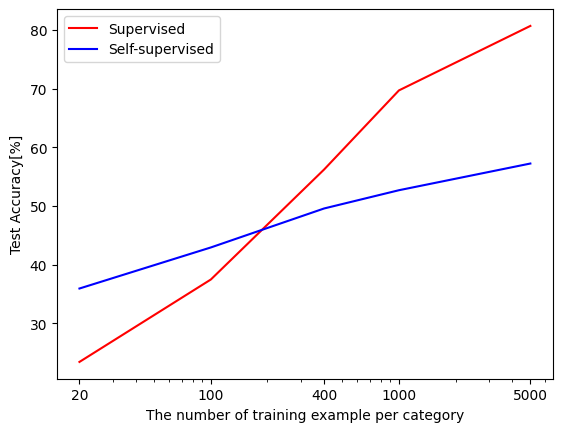
\includegraphics[scale = 0.4]{"fig/extracredit.png"}
    \end{center}
    \caption{The test accuaracy of the both supervised model and self-supervised model with respect to the amount of accessible training data. }
    \label{fig4}
\end{figure}

\begin{table}[!h]
    \begin{center}
        \begin{tabular}{ccc}
            \textbf{\# of training data} & \textbf{Supervised} & \textbf{Self-supervised} \\ \hline
            20                           & 21.61               & 34.62                    \\
            100                          & 38.44               & 48.74                    \\
            400                          & 60.05               & 53.38                    \\
            1000                         & 69.02               & 56.62                    \\
            5000                         & 80.36               & 59.94                   
            \end{tabular}
    \end{center}
    \caption{The test score of supervised and self-supervised model}
\end{table}

In alignment with the experimental findings presented by Gidaris et al. (2018), it is observed that the self-supervised model consistently outperforms its supervised counterpart, specifically under conditions where the available training data is limited or scarce. This particular performance comparison is illustrated in Figure \ref{fig4}, which provides a visual representation of the superiority of the self-supervised model in such challenging conditions.
The significance of this finding lies in highlighting the potential of the self-supervised model in a semi-supervised learning environment. As a matter of fact, it brings to light the model's capacity to learn and improve even with a small amount of labeled data, therefore compensating for the lack of abundant training data. This is particularly beneficial in real-world applications where obtaining large amounts of labeled data can be expensive, time-consuming, or practically impossible.


\appendix
\section{Plotting Code}
\begin{python}
import time

def run_test(net, testloader, criterion, task):
    correct = 0
    total = 0
    avg_test_loss = 0.0
    with torch.no_grad():
        for images, images_rotated, labels, cls_labels in testloader:
            if task == 'rotation':
              images, labels = images_rotated.to(device), labels.to(device)
            elif task == 'classification':
              images, labels = images.to(device), cls_labels.to(device)
            outputs = net(images)
            predicted = torch.max(outputs.data,1)[1]

            total += labels.size(0)
            correct += (predicted == labels).sum().item()
            avg_test_loss += criterion(outputs, labels)  / len(testloader)
    print('TESTING:')
    print(f'Accuracy of the network on the 10000 test images: {100 * correct / total:.2f} %')
    print(f'Average loss on the 10000 test images: {avg_test_loss:.3f}')
    return avg_test_loss.item(), 100*correct/total

def train(net, criterion, optimizer, num_epochs, decay_epochs, init_lr, task):
    logger = {
        'train_loss' :[],
        'train_acc' :[],
        'test_loss' : [],
        'test_acc' : []
    }
    for epoch in range(num_epochs):  # loop over the dataset multiple times

        running_loss = 0.0
        running_correct = 0.0
        running_total = 0.0
        start_time = time.time()
        net.train()
        train_logger = {'loss' : [], 'acc' : []}

        for i, (imgs, imgs_rotated, rotation_label, cls_label) in enumerate(trainloader, 0):
            adjust_learning_rate(optimizer, epoch, init_lr, decay_epochs)
            if task == "rotation":
              images, labels = imgs_rotated.to(device), rotation_label.to(device)
            elif task == "classification":
              images, labels = imgs.to(device), cls_label.to(device)
            optimizer.zero_grad()
            output = net(images)
            loss = criterion(output, labels)
            loss.backward()
            optimizer.step()
            predicted = torch.max(output.data,1)[1]
            print_freq = 100
            running_loss += loss.item()
            running_total += labels.size(0)
            running_correct += (predicted == labels).sum().item()

            if i % print_freq == (print_freq - 1):    # print every 2000 mini-batches
                print(f'[{epoch + 1}, {i + 1:5d}] loss: {running_loss / print_freq:.3f} acc: {100*running_correct / running_total:.2f} time: {time.time() - start_time:.2f}')
                running_loss, running_correct, running_total = 0.0, 0.0, 0.0
                start_time = time.time()

        logger['train_loss'].append(running_loss/print_freq)
        logger['train_acc'].append(100*running_correct/running_total)

        net.eval()
        test_loss, test_acc = run_test(net, testloader, criterion, task)

    logger['test_loss'].append(test_loss)
    logger['test_acc'].append(test_acc)
    print('Finished Training')
    return logger

logger = train(net, criterion, optimizer, num_epochs=45, decay_epochs=15, init_lr=0.01, task='rotation')

fig, ax1 = plt.subplots()

line1 = ax1.plot(range(45),logger['train_loss'],label = "train loss",color = 'k',ls = '-')
ax1.set_xlabel('Epoch')
ax1.set_ylabel('Loss')

ax2 = ax1.twinx()
line2 = ax2.plot(range(45),logger['train_acc'],label = "train accuracy",color = 'k', ls = '--')
ax2.set_xlabel('Epoch')
ax2.set_ylabel('Accuracy[%]')

lines = [line1[0], line2[0]]
labels = [line.get_label() for line in lines]
ax1.legend(lines, labels, loc='center right')

print("Test Loss : ", logger['test_loss'])
print("Test Accuracy : ", logger['test_acc'])

\end{python}

\bibliographystyle{unsrt}
\bibliography{ref.bib}

\end{document}